\chapter{Introduction}
%Investigating matter with light is one of the most fundamental approaches to study nature. Whether we look at things by eye or use more advanced methods for example using lasers, it is an invaluable tool to understand nature. Through light, we can study the shapes of objects, investigate fundamental particles, study quantum mechanics and so much more. Key aspect in almost any study involving light is it's wavelength. The wavelength of light can make you feel cozy at home with a modern LED light bulb or shroud your home in a blue, uncomfortable haze when you use older light bulbs. At the end of the 19th century, R\"ontgen discovered the then novel X-radiation and quickly realized its impact due to its different wavelength. Soon, he was able to take first medical X-ray images, later X-rays could be used to investigate fundamental aspects of atoms. The success story continues until today, where short wavelength X-rays enables the study of the workhorse in human bodies, namely proteins. The shape of a protein, which is only a few nanometers in size, cannot be seen in a microscope anymore and only X-rays can be used to unravel their shape with sufficient resolution. The shape of a biomolecules is of particular interest because it defines its biological function. The chemical structure of most human biomolecules are fairly similar and affect the function little. Medical drugs often aim to affect biological functions such that the specific shape of a protein becomes very important for drug research and drug design. \\
% R\"ontgen discovered the X-radiation \citep{Roentgen-NP} and quickly realized its impact due to its novel attributes. Soon, he was able to take the first medical X-ray image.
Following the discovery of \textit{X-radiation} at the end of the 19$^{\text{th}}$ century by R\"ontgen \cite{Roentgen-NP}, X-rays have been used to understand and investigate matter in unprecedented ways. Soon after this discovery, X-rays were used to take the first medical image. Later, X-rays led to the understanding of fundamental aspects of atoms \citep{Siegbahn-NP} and crystals \citep{Laue-NP,Bragg-NP}. Today, the success story continues in various fields of science. A large and active scientific field is structural biology. Here, X-rays are being used to study the structure of proteins through crystallography. Proteins are the so-called ``workhorse'' in the human body and the structure of a protein defines its biological function. Unfortunately not all proteins can be grown into large crystals making the molecular structure determination challenging. However, new lightsources, namely \textit{X-ray free electron lasers} (XFELs) \citep{Ackermann-2007-NPho} have more and more peak \textit{brightness} allowing the structure determination of smaller and smaller protein-crystals \citep{Chapman-2011-Nature}.\\[1\baselineskip]
%
The first hard XFEL was built at Stanford University and is called the Linac Coherent Light Source (LCLS) \citep{Emma-2010-NatPho}. It is a multikilometer long machine that produces X-rays with wavelengths from \SIrange{4.6}{0.1}{\nano\meter}, has intensities of up to \SI{\sim e18}{\watt\per\square\centi\meter}, and has ultra-short pulses ranging from \SIrange{1}{500}{\femto\second}. Scientists from various disciplines can apply to use this lightsource for their experiments, which are conducted in several instruments. The Atomic, Molecular, and Optical physics (AMO) instrument at the LCLS was the first of seven instruments in operation and is a focal point for experiments ranging from biological imaging to basic science \citep{Bostedt-2016-RMP}.\\[1\baselineskip]
%
The beam parameters that are available at the AMO instrument opened up an entirely new method for structural biologists, which is the \textit{single particle imaging} (SPI). With SPI (see Figure \ref{fig:spi-concept}), the shape of single bio-molecules can be determined through \textit{diffractive imaging} \citep{Chapman-2006-NatPhys}. First experiments have successfully delivered single-shot diffraction images of biological particles, such as viruses \citep{Seibert-2011-Nature} and non-biological particles, such as rare-gas clusters \citep{Gomez-2014-Science}. It has been a rapidly developing field that has recently succeeded in visualizing 3D images of nano-objects \citep{Ekeberg-2015-PRL,Barke-2015-NatComm}.\\[1\baselineskip]
%
%All matter irradiated by intense X-ray radiation disintegrates into its atomic components on ultrafast\footnote{Ultrafast timescales are on the order of atto- to nanoseconds.} timescales \citep{Neutze-2000-Nature}. This process is a form of \textit{radiation damage} and is a major challenge for imaging methods with XFEL \citep{Aquila-2015-StrucDyn}.
%So, the underlying principle of diffractive imaging is that intense X-ray pulses diffract from a single macromolecular structure before they destroy it.\\[1\baselineskip]
%
%Imagine now that we expose a nanoparticle to the highly intense X-rays from LCLS. Within the first moment of light-nanoparticle interaction, photons elastically scatter in an angular distribution distinctive to the shape of the particle that we are able measure in 2D. However, the particle will also absorb the rays from the first moment on, which leads to inner atomic-shell vacancies \citep{Young-2010-Nature}. Subsequent processes, such as the \textit{Auger-decay}, occur only a few femtoseconds later and eventually the nanoparticle is transformed into a \textit{nanoplasma}. Several forces will expand the plasma on a femtosecond timescale \citep{Gorkhover-2016-NatPho}. Finally, the nanoplasma disintegrates into its atomic components. The absorption process, which triggers this cascade of events in the nanoparticle, is unavoidable when the particle is exposed to intense X-rays and so is radiation damage in the sample.\\[1\baselineskip]
\begin{figure}
	\centering
		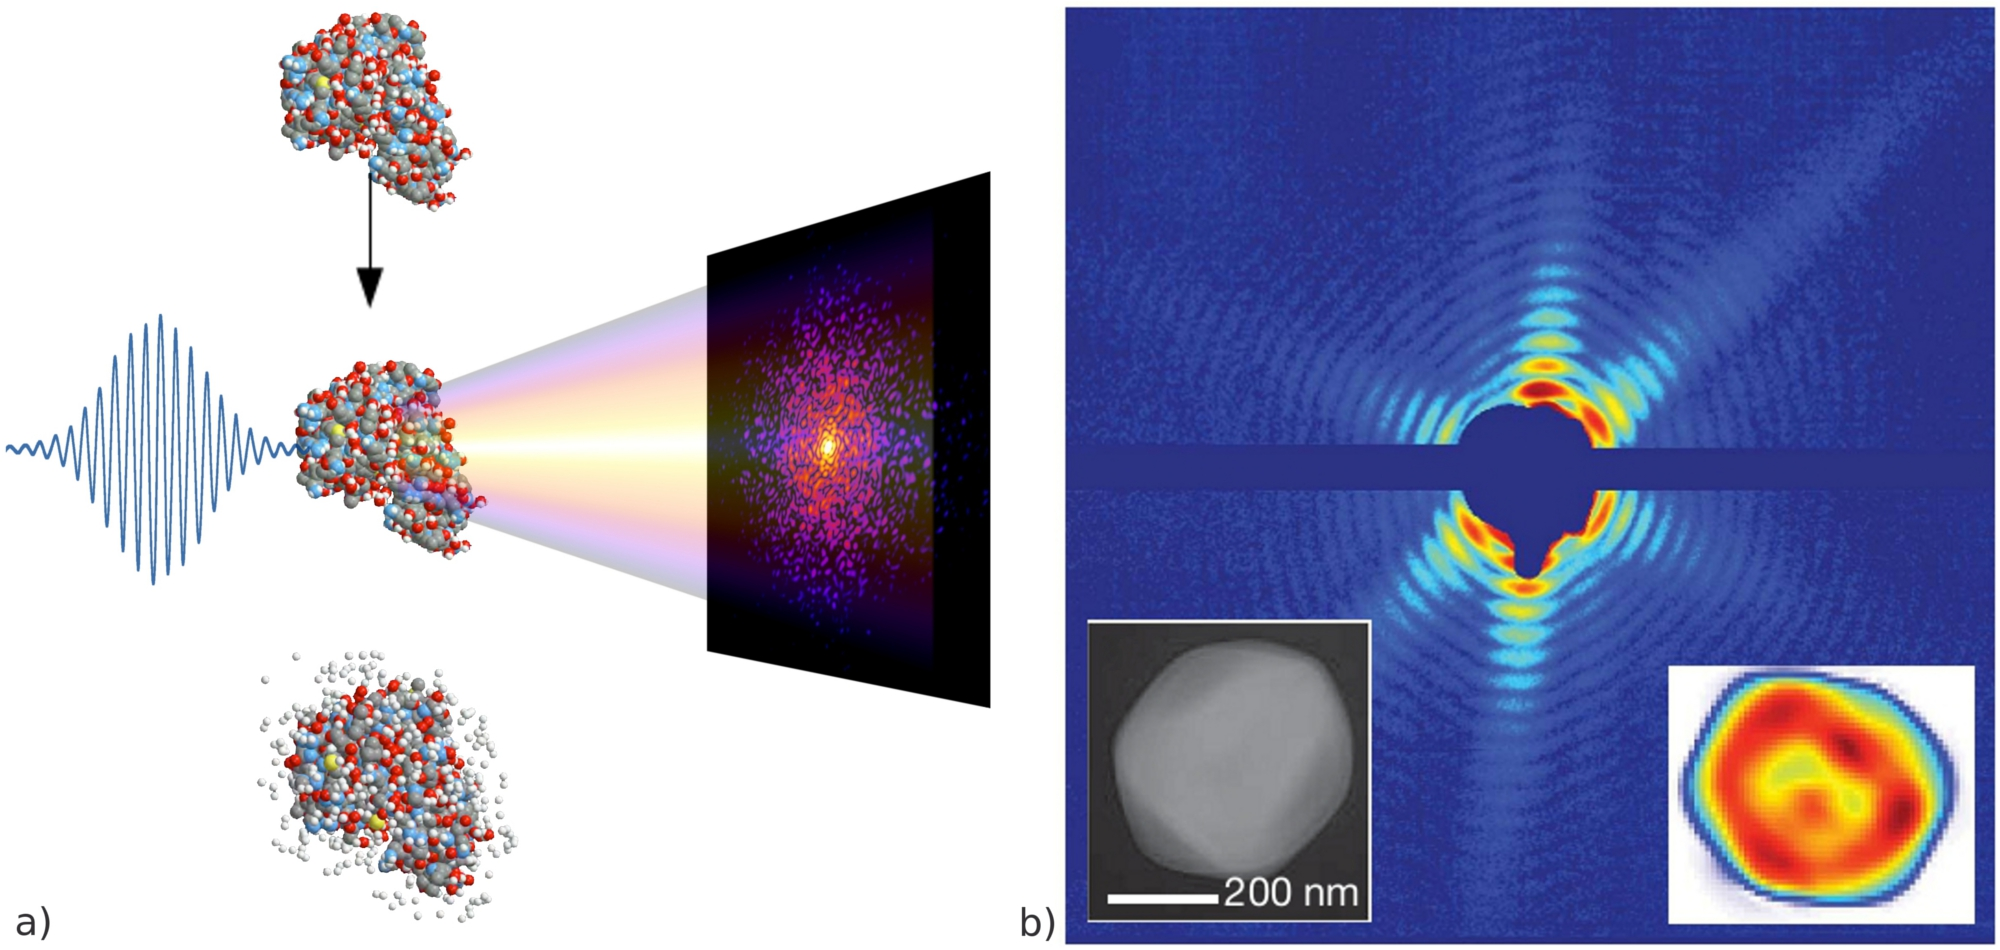
\includegraphics[width=0.80\textwidth]{images/intro-dani.jpg}
	\caption[Conceptual setup of a single particle imaging experiment.]{a) Conceptual setup of a single particle imaging experiment. A nanoparticle is injected and intercepted by an XFEL pulse. The nanoparticle scatters before it is destroyed and the scattering is recorded with a detector. b) Single-shot diffraction image and reconstruction (right inset) of a single Mimivirus. A electron-microscopy image is show as comparison  (left inset). From \cite{Rupp-2013-Thesis,Neutze-2000-Nature,Seibert-2011-Nature}.}
	\label{fig:spi-concept}
\end{figure}
%
But the highly-intense pulses that enable diffractive imaging lead to unusual questions. When an intense soft X-ray pulse irradiates a nanoparticle, the particle will simultaneously absorb and diffract X-rays with the absorption cross-section being much larger than the scattering cross-section. From the first moment of light-matter interaction, the absorption will lead to inner atomic-shell vacancies \citep{Young-2010-Nature} and these vacancies make the above cross-sections time-dependent. Subsequent \textit{core-hole decays}, such as the \textit{Auger decay}, occur only a few femtoseconds later and the nanoparticle is thus transformed into a \textit{nanoplasma} on a femtosecond timescale. Several forces will expand the plasma \citep{Gorkhover-2016-NatPho} until eventually, the nanoplasma disintegrates into its atomic components.\\[1\baselineskip]
%
The underlying principle of diffractive imaging, which is that intense X-ray pulses diffract from a single macromolecular structure before they destroy it\footnote{This is often referred to as ``diffraction before destruction''.} \cite{Neutze-2000-Nature}, is now challenging since sample damage occurs while the X-ray pulse propagates through the nanoparticle \cite{Aquila-2015-StrucDyn}. Changing scattering factors and trapped, or delocalized electrons will affect the diffraction image. While diffractive imaging is still feasible, these fundamental processes will limit the achievable resolution in single particle imaging. Several ideas have been proposed to address radiation damage in single particle imaging: Computer models can account for known processes \citep{Quiney-2010-NatPhys}; molecule alignment prior imaging provides additional information \citep{Kupper-2014-PRL}; and sacrificial layers slow the nanoplasma expansion by transferring charges from the photoionized sample and transporting kinetic energy away from the sample (see Figure \ref{fig:tamper-layer}) \citep{Hau-Riege-2004-PRE,Hau-Riege-2010-PRL,Hoener-2008-JPB}. While experimental data exist for the first two ideas, sacrificial layers have not yet been used on aerosol injected particles and studied experimentally using diffractive imaging. This is a key aspect of this thesis work.\\[1\baselineskip]
%The principle of ``outrunning'' the radiation induced damage with femtosecond lightpulses is challenging for two reasons. One, it limits the intensity output of the lightsource, and two, sample damages due to photoionization and changing scattering factors are inevitable. 
%Ultimately, these reasons will limit the achievable resolution in single-particle imaging. But radiation damage can also be addressed in other ways. Computer models can account for known processes \citep{Quiney-2010-NatPhys} and novel methods from AMO physics, such as molecule alignment \citep{Kupper-2014-PRL} and sacrificial tamper layers \citep{Hau-Riege-2004-PRE,Hau-Riege-2010-PRL} may inhibit it.\\[1\baselineskip]
%
\begin{figure}
	\centering
		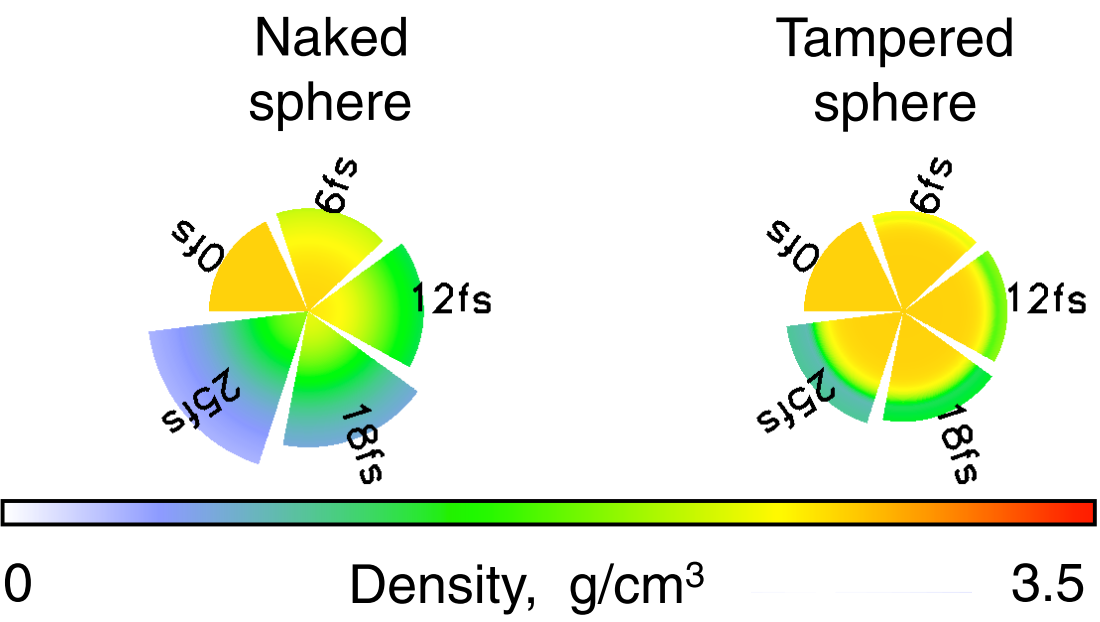
\includegraphics[width=0.80\textwidth]{images/tamper-layer.png}
	\caption[Computer simulations of aluminum spheres with tamper layers]{Computer simulations of \SI{7.5}{\nano\meter} radius aluminum spheres that are illuminated by intense soft X-rays with a fluence of \SI{2.5e8}{\joule\per\square\centi\meter}. On the left is a pristine Al-sphere and on the right is a Al-sphere with a \SI{2.5}{\nano\meter} thick silicon tamper layer. From \citep{Hau-Riege-2010-PRL}. Reprinted with permission from APS.}
	\label{fig:tamper-layer}
\end{figure}
%
%Sacrificial layers, or tamper layers, supply electrons to the photoionized sample and transport kinetic energy away from the sample. This reduces the ionization level of the sample
An effective tamper layer would ideally be thin and uniform around the sample to minimize its background signal. The initial idea of a sacrificial layer material was water, since bio-molecules are typically embedded in water-based layers when injected into typical diffractive imaging setups using an aerosol sample jet. However, water-based tampers become disordered in thicker layers and are usually uneven around macro-molecules \cite{Aquila-2015-StrucDyn}. Recently, helium layers have been proposed as a tamper material \cite{Mikaberidze-2008-PRA}. Currently, aerosol sample jets use helium to dry the injected sample before injection and a next step that is discussed, is to equip a sample with a helium tamper during the injection process.\\[1\baselineskip]
%An alternative is to use helium-based layers, whereby, for example, a sample particle is placed inside a helium-droplet.
%
This thesis discusses experimental data of sacrificial layers that are in the form of a helium-droplet, which has xenon-clusters embedded. Thereby act the Xe-clusters as a testbed sample. The data are complemented by the study of pristine Xe- and He-clusters. A novel \textit{X-ray pump--X-ray probe} method was employed to study the nanoplasma formation in those samples. Here, the pump-pulse triggers the nanoplasma formation and the probe-pulse creates a ``snapshot'' of the system at a later time. Coincident diffraction images and time-of-flight mass spectra are measured and further analyzed. Real-space reconstructions of the clusters are shown with thus far unprecedented resolution and allow to answers the following questions:
\begin{itemize}
	%\item How does X-ray induced damage compare to optical light induced damage?
	%\item On what timescales do absorption cross-sections change due to X-ray irradiation?
	\item How does an X-ray induced nanoplasma-formation affect the shape of Xe-clusters?
	%\item On what timescales are diffraction images affected at current resolution?
	\item How do mixed HeXe-clusters self-organize as nanoparticles?
	\item Does helium compare to sacrificial tamper layers in mixed HeXe-clusters?
\end{itemize}
%
This document is organized as follows: Chapter \ref{ch:fundamental_concepts} discusses fundamental aspects that are used throughout this study; Chapter \ref{ch:exp_setup} describes the experimental setup at the AMO instrument at LCLS and in particular the LAMP end-station with it's detectors; Chapter \ref{ch:methods} discusses several computational methods; Chapter \ref{ch:results} presents the results of the pump--probe study; and Chapter \ref{ch:summary_outlook} summarizes the present work and provides an outlook for further studies.
%
%
%